\documentclass[aspectratio=169]{beamer}
%\documentclass[aspectratio=43]{beamer}

\usepackage{graphicx}  % Required for including images
\usepackage{natbib}
\usepackage{booktabs} % Top and bottom rules for tables
\usepackage{amssymb,amsthm,amsmath}
\usepackage{exscale}
\usepackage{natbib}
\usepackage{tikz}
\usepackage{listings}
\usepackage{color}
\usepackage{animate}
\usepackage{bm}
\usepackage{etoolbox}

% Setup TikZ
\usepackage{tikz}
\usetikzlibrary{arrows}
\tikzstyle{block}=[draw opacity=0.7,line width=1.4cm]
% Setup hyperref
\usepackage{hyperref}
\hypersetup{colorlinks=true}
\hypersetup{citecolor=porange}
\hypersetup{urlcolor=porange!80!}
\hypersetup{linkcolor=porange}

\newtheorem{proposition}{Proposition}
\newtheorem{remark}{Remark}
\newtheorem{principle}{Principle}

%% Writing quarters
\newcommand{\wQ}[1]{{\textcolor{white}{Q#1}}}
\newcommand{\bQ}[1]{{Q#1}}

% Uncomment appropriate command to disable/enable hiding
%\newcommand{\mypause}{\pause}
\newcommand{\mypause}{}
\newcommand{\myb}[1]{{\color{blue} {#1}}}

%% Commonly used macros
\newcommand{\eqr}[1]{Eq.\thinspace(#1)}
\newcommand{\pfrac}[2]{\frac{\partial #1}{\partial #2}}
\newcommand{\pfracc}[2]{\frac{\partial^2 #1}{\partial #2^2}}
\newcommand{\pfraca}[1]{\frac{\partial}{\partial #1}}
\newcommand{\pfracb}[2]{\partial #1/\partial #2}
\newcommand{\pfracbb}[2]{\partial^2 #1/\partial #2^2}
\newcommand{\spfrac}[2]{{\partial_{#1}} {#2}}
\newcommand{\mvec}[1]{\mathbf{#1}}
\newcommand{\gvec}[1]{\boldsymbol{#1}}
\newcommand{\script}[1]{\mathpzc{#1}}
\newcommand{\eep}{\mvec{e}_\phi}
\newcommand{\eer}{\mvec{e}_r}
\newcommand{\eez}{\mvec{e}_z}
\newcommand{\iprod}[2]{\langle{#1}\rangle_{#2}}

\DeclareMathAlphabet{\mathpzc}{OT1}{pzc}{m}{it}

%% Autoscaled figures
\newcommand{\incfig}{\centering\includegraphics}
\setkeys{Gin}{width=0.9\linewidth,keepaspectratio}

%Make the items smaller
\newcommand{\cramplist}{
	\setlength{\itemsep}{0in}
	\setlength{\partopsep}{0in}
	\setlength{\topsep}{0in}}
\newcommand{\cramp}{\setlength{\parskip}{.5\parskip}}
\newcommand{\zapspace}{\topsep=0pt\partopsep=0pt\itemsep=0pt\parskip=0pt}

\newcommand{\backupbegin}{
   \newcounter{finalframe}
   \setcounter{finalframe}{\value{framenumber}}
}
\newcommand{\backupend}{
   \setcounter{framenumber}{\value{finalframe}}
}

\usetheme[bullet=circle,% Use circles instead of squares for bullets.
          titleline=true,% Show a line below the frame title.
          ]{Princeton}

\title[{\tt }]{Hyperbolic PDEs and Finite-Volume Methods II}%
\author[https://ast560.rtfd.io]%
{Ammar H. Hakim ({\tt ammar@princeton.edu}) \inst{1}}%

\institute[PPPL]
{ \inst{1} Princeton Plasma Physics Laboratory, Princeton, NJ %
}

\date[3/11/2021]{Princeton University, Course AST560, Spring 2021}

\begin{document}

\begin{frame}[plain]
  \titlepage
\end{frame}

\begin{frame}{Hyperbolic PDEs: rigorous definition, no reliance on
    linearization}
  Consider a system of conservation laws written as
  \begin{align*}
    \pfrac{\mvec{Q}}{t} + \pfrac{\mvec{F}}{x} = 0.
  \end{align*}
  where $\mvec{Q}$ is a vector of conserved quantities and
  $\mvec{F}(\mvec{Q})$ is a vector of fluxes. This system is called
  \emph{hyperbolic} if the flux Jacobian
  \begin{align*}
    \mvec{A} \equiv \pfrac{\mvec{F}}{\mvec{Q}}
  \end{align*}
  has \emph{real eigenvalues} and a \emph{complete set of linearly
    independent} eigenvectors. In multiple dimensions if $\mvec{F}_i$
  are fluxes in direction $i$ then we need to show that arbitrary
  linear combinations
  $\sum_i n_i {\partial\mvec{F}_i}/{\partial\mvec{Q}}$ have real
  eigenvalues and linearly independent set of eigenvectors.
  
\end{frame}

\begin{frame}{The Riemann Problem for hyperbolic PDEs}
  \small%
  The Riemann problem is a class of \emph{initial value} problems for
  a hyperbolic PDE
  \begin{align*}
    \pfrac{\mvec{Q}}{t} + \pfrac{\mvec{F}}{x} = 0.
  \end{align*}
  on $x\in[-\infty,\infty]$ with initial conditions
  \begin{align*}
    \mvec{Q}(x,0) = \mvec{Q}_R \quad x>0 \\
    \mvec{Q}(x,0) = \mvec{Q}_L \quad x<0    
  \end{align*}
  where $\mvec{Q}_{L,R}$ are \emph{constant} initial states.%
  \mypause%
  \begin{itemize}
  \item Fundamental mathematical problem in theory of hyperbolic PDEs:
    brings out the key structure of the nonlinear solutions of the
    system.
  \item For some important systems like (relativisitic) Euler
    equations, ideal MHD the Riemann problem can be solved
    \emph{exactly} (modulo some nonlinear root-finding).
  \item Good test for shock-capturing schemes as it tests ability to
    capture discontinuities and complex non-linear phenomena.
  \end{itemize}
\end{frame}  

\begin{frame}{Weak-solutions and entropy conditions}
  \footnotesize%
  At a shock the solution has a discontinuity. Hence, derivatives are
  not defined! Differential form of the equations break-down. We must
  use concept of weak-solutions in this case.%
  \vskip0.1in%
  Let $\phi(x,t)$ is a compactly supported (i.e. zero outside some
  bounded region) smooth function (enough continuous
  derivatives). Then multiply conservation law
  \begin{align*}
    \int_0^\infty  \int_{-\infty}^\infty \phi(x,t)
    \bigg[\pfrac{\mvec{Q}}{t} + \pfrac{\mvec{F}}{x}\bigg]\thinspace
    dx\thinspace dt = 0
  \end{align*}
  by $\phi(x,t)$ and integrating by parts to get the \emph{weak-form}
  \begin{align*}
    \int_0^\infty  \int_{-\infty}^\infty 
    \bigg[\pfrac{\phi}{t} \mvec{Q} + \pfrac{\phi}{x} \mvec{F}\bigg]\thinspace
    dx\thinspace dt
    =
    -
    \int_{-\infty}^\infty \phi(x,0) \mvec{Q}(x,0) dx.
  \end{align*}  
  \begin{definition}[Weak-solution]
    A function $\mvec{Q}(x,t)$ is said to be a weak-solution if it
    satisfies the weak-form for all compact, smooth $\phi(x,t)$.
  \end{definition}
  
\end{frame}

\begin{frame}{Weak-solutions and entropy conditions}
  Unfortunately, weak-solutions are not unique! Why does this happen?
  \vskip0.1in%
  In physical problems there is always some non-ideal effects
  (viscosity, Landau damping etc) that does not allow a genuine
  discontinuity to form. However, this ``viscous shock layer'' can be
  extremely thin compared to system size. Also, we know entropy must
  increase in the physical universe.

  \vskip0.1in%
  This indicates we can recover uniqueness in two ways
  \begin{itemize}
  \item {\color{gray}{Add a viscous (diffusion) term and take limit of
      viscosity going to zero. (Generally not convenient for numerical
      work)}}%
  \item Impose \emph{entropy condition}: construct an \emph{entropy}
    function such that it remains conserved for smooth solutions but
    \emph{increases} across a shock. Entropy is naturally suggested in
    most physical problems.
  \end{itemize}  
\end{frame}

\begin{frame}{Weak-solutions of Burgers' equation: shock}
  \small%
  When characteristics \emph{converge} a shock will form
  \begin{figure}
    \setkeys{Gin}{width=0.75\linewidth,keepaspectratio}
    \incfig{burgers-shock.pdf}
  \end{figure}  
\end{frame}

\begin{frame}{Shock-speed is given by the Rankine-Hugoniot jump
    condition}
  \small%
  Consider a discontinuity in the solution wirh left/right states
  $\mvec{Q}_L$ and $\mvec{Q}_R$. Then the speed at which this
  discontinuity moves, $s$, is called the \emph{shock-speed} and is
  determined by the Rankine-Hugoniot jump condition
  \begin{align*}
    s(\mvec{Q}_R-\mvec{Q}_L) = \mvec{F}_R-\mvec{F}_L
  \end{align*}
  For Burgers's equation we simply have
  \begin{align*}
    s = \frac{1}{2}(u_L + u_R).
  \end{align*}
  For linear systems of hyperbolic equations as
  $\mvec{F} = \mvec{A}\mvec{Q}$ we have
  \begin{align*}
    s(\mvec{Q}_R-\mvec{Q}_L) = \mvec{A}(\mvec{Q}_R-\mvec{Q}_L)
  \end{align*}
  which means the eigenvalues of $\mvec{A}$ are the shock-speeds.%
  \vskip0.1in%
  For general nonlinear hyperbolic systems only very specific jumps in
  which the jump in flux and jump in conserved variables are
  \emph{linearly dependent} can be shocks.
\end{frame}

\begin{frame}{Weak-solutions of Burgers' equation: rarefaction}
  \small%
  When characteristics \emph{diverge} inifinite solutions to the
  weak-form! An entropy respecting solution is a \emph{rarefaction}
  \begin{figure}
    \setkeys{Gin}{width=0.75\linewidth,keepaspectratio}
    \incfig{burgers-rarefaction.pdf}
  \end{figure}
  One possible defintion of entropy respecting shocks for Burgers'
  equation: \emph{only} allow a discontinuity if $u_L > u_R$. So in
  the above case me must not allow a shock to form.
\end{frame}  

\begin{frame}{Weak-solutions: shock and rarefaction}
  \small%
  When characteristics \emph{diverge} (right plot below) the
  weak-solution is not unique. A false ``shock'' solution also is a
  weak-solution. Imposing \emph{entropy condition} gives a
  \emph{rarefaction} wave seen in the right plot.
  \begin{columns}
    \begin{column}{0.5\textwidth}
      \begin{figure}
        \setkeys{Gin}{width=1.0\linewidth,keepaspectratio}
        \incfig{burgers-step-a.png}
      \end{figure}      
    \end{column}
    \begin{column}{0.5\textwidth}
      \begin{figure}
        \setkeys{Gin}{width=1.0\linewidth,keepaspectratio}
        \incfig{burgers-step-b.png}
      \end{figure}
    \end{column}
  \end{columns}  
\end{frame}

\begin{frame}{Euler equations of invicid fluids}
  \small%
  The Euler equations for invicid fluids are important in themselves,
  and form the basis of many other more complex equation systems
  (Navier-Stokes, multi-fluid plasma equations, MHD, ...)
  \begin{align*}
    \pfrac{\rho}{t} + \nabla\cdot(\rho\mvec{u}) &= 0 \qquad{\textrm{Continuity}} \\
    \pfrac{(\rho\mvec{u})}{t} +
    \nabla\cdot(\rho\mvec{u}\mvec{u} + p\mvec{I}) &= 0
                                                    \qquad{\textrm{Momentum}}
    \\
    \pfrac{\mathcal{E}}{t} + \nabla\cdot\left[(\mathcal{E}+p)\mvec{u}
    \right] &= 0
              \qquad{\textrm{Energy}}
  \end{align*}
  where
  \begin{align*}
    \mathcal{E} =
    \underbrace{\frac{p}{\gamma-1}}_{\textrm{IE}} +
    \underbrace{\frac{1}{2}\rho u^2}_{\textrm{KE}}
    .
  \end{align*}
  is the total energy of the system. If we solve the system in this
  \emph{conservative} form, then density, momentum and energy are
  conserved automatically, even locally.
\end{frame}  

\begin{frame}{Euler equations: hyperbolicity}
  \begin{align*}
    \frac{\partial}{\partial{t}}    
    \left[
    \begin{matrix}
      \rho \\
      \rho u \\
      \rho v \\
      \rho w \\
      \mathcal{E}
    \end{matrix}
    \right]
    +
    \frac{\partial}{\partial{x}}
    \left[
    \begin{matrix}
      \rho u \\
      \rho u^2 + p \\
      \rho uv \\
      \rho uw \\
      (\mathcal{E}+p)u
    \end{matrix}
    \right]
    =
    0    
  \end{align*}
  Here $\mathcal{E} = p/(\gamma-1) + \rho u^2/2$ is the total
  energy. Eigenvalues of this system are $\{u-c_s,u,u,u,u+c_s \}$
  where $c_s = \sqrt{\gamma p/rho}$ is the sound speed. See class
  notes for left/right eigenvectors.%
  \vskip0.1in%
  Note: in the limit $p\rightarrow 0$ all eigenvalues become $u$ and
  for cold-fluid ($p=0$) the system does not possess complete set of
  eigenvectors. (Cold fluid model is important in plasmas and to model
  dust, for example, in astrophysical systems or in say volcanic
  explosions).
\end{frame}

\begin{frame}{Euler equations: transport of kinetic energy}
  \footnotesize%
  The energy conservation equation for Euler equation is
  \begin{align*}
    \pfrac{\mathcal{E}}{t} + \nabla\cdot\left[(\mathcal{E}+p)\mvec{u} \right] = 0
  \end{align*}
  where
  \begin{align*}
    \mathcal{E} =
    \underbrace{\frac{p}{\gamma-1}}_{\textrm{IE}} +
    \underbrace{\frac{1}{2}\rho u^2}_{\textrm{KE}}
    .
  \end{align*}
  \mypause%
  We can derive instead \emph{balance laws} (not conservation laws)
  for transport of KE and IE
  \begin{align*}
    \pfraca{t}(\textrm{KE})
    +
    \nabla\cdot(\textrm{KE}\thinspace \mvec{u} )
    &=
      -\mvec{u}\cdot\nabla p \\
    \pfraca{t}(\textrm{IE})
    +
    \nabla\cdot(\textrm{IE}\thinspace \gamma\mvec{u} )
    &=
      \mvec{u}\cdot\nabla p    
  \end{align*}
  \mypause%
  It is important to ensure that in the \emph{numerics} exchange of
  kinetic and internal energy is only via the RHS terms (pressure
  work).%
  \vskip0.1in%
  Many shock-capturing and higher-order methods can mess this up for
  high-$k$ (short wavelength) modes due leading to incorrect energy
  spectra. (No Free Lunch Principle).
\end{frame}

\begin{frame}{Euler equations: shocks, rarefactions and contacts}
  In addition to shocks and rarefactions which we saw in Burgers's
  equation, Euler equations also support \emph{contact
    discontinuities}, across which density has a jump but not pressure
  or velocity.
  \begin{figure}
    \setkeys{Gin}{width=0.33\linewidth,keepaspectratio}
    \incfig{sod-density.png}
    \incfig{sod-pressure.png}
    \incfig{sod-vel.png}    
  \end{figure}    
\end{frame}

\begin{frame}{Beyond hyperbolic PDEs: Source terms, non-ideal effects}
  In most physics applications one must add source terms and non-ideal
  effects to the underlying hyperbolic PDE, converting it into a PDE
  of \emph{mixed} type. Typically we will have systems of the form
  \begin{align*}
    \pfrac{\mvec{Q}}{t} + \pfrac{\mvec{F}}{x} + \pfrac{\mvec{G}}{x}
    + \ldots
    = \mvec{S}
  \end{align*}
  where $\mvec{G}(\mvec{Q},\partial\mvec{Q}/\partial x)$ are
  \emph{viscous}/non-ideal fluxes that depend on \emph{gradients} of
  $\mvec{Q}$ (viscous stress-tensor in Navier-Stokes equations,
  heat-conducion etc) and $\mvec{S}(\mvec{Q},x,t)$ are \emph{source}
  terms.%
  \vskip0.1in%
  The presence of non-ideal and source terms can \emph{significantly}
  change the physics and required numerics.
\end{frame}

\begin{frame}{Example: Ideal multifluid equations (five-moment)}
  Multi-fluid plasma equations are an important example. Ignoring
  non-ideal terms:
  \begin{align*}
    \pfrac{\rho_s}{t} + \nabla\cdot(\rho_s\mvec{u}_s) &= 0 \\
    \pfraca{t}(\rho_s\mvec{u}_s) + \nabla\cdot(\rho_s\mvec{u}_s\mvec{u}_s + p_s\mvec{I})
                                                      &=
                                                        \frac{q_s\rho_s}{m_s}(\mvec{E} + \mvec{u}_s\times \mvec{B})
    \\
    \pfrac{\mathcal{E}_s}{t} + \nabla\cdot\left[(\mathcal{E}_s+p_s)\mvec{u}_s
    \right] &= \frac{q_s\rho_s}{m_s}\mvec{u}_s\cdot\mvec{E}
  \end{align*}
  for each plasma species $s$ (electrons, ions, ...). These are
  coupled to Maxwell equations
  \begin{align*}
    \frac{\partial \mathbf{B}}{\partial t} + \nabla \times \mathbf{E}
    &= 0 \\
    \epsilon_0 \mu_0 \frac{\partial \mathbf{E}}{\partial t} - \nabla
    \times \mathbf{B} &= -\mu_{0}\sum_s \frac{q_s\rho_s}{m_s}\mvec{u}_s
  \end{align*}
\end{frame}

\begin{frame}{Multifluid equations (five-moment): conservation
    properties}
  Note that in multifluid system total momentum (fluid+field) and
  total energy (fluid+field) is conserved. Hence, conservation
  properties are \emph{indirect}: ensuring conservation of total
  momentum and total energy (specially locally) is non-trivial.
  \footnotesize
  \begin{align*}
    \pfraca{t}
    \left(
    \sum_s \rho_s\mvec{u}_s + \epsilon_0 \mvec{E}\times\mvec{B}
    \right)
    + \nabla\cdot
    \left[
    \sum_s (\rho_s\mvec{u}_s\mvec{u}_s + p_s\mvec{I})
    +
    \left(
    \frac{\epsilon_{0}}{2}|\mathbf{E}|^{2}+\frac{1}{2
    \mu_{0}}|\mathbf{B}|^{2}
    \right)\mvec{I}
    -
    \left(
    \epsilon_{0} \mathbf{E E}+\frac{1}{\mu_{0}} \mathbf{B B}
    \right)
    \right]
    = 0
  \end{align*}
  \begin{align*}
    \pfraca{t}
    \left(
    \sum_s \mathcal{E}_s + \frac{\epsilon_{0}}{2}|\mathbf{E}|^{2}+\frac{1}{2 \mu_{0}}|\mathbf{B}|^{2}
    \right)
    + \nabla\cdot\left[
    \sum_s (\mathcal{E}_s+p_s)\mvec{u}_s
    +
    \frac{1}{\mu_0} \mvec{E}\times\mvec{B}
    \right]
    = 0.
  \end{align*}    
\end{frame}  

\begin{frame}{Multifluid equations (five-moment): eigensystem}
  \small%
  \begin{columns}  
    \begin{column}{0.5\linewidth}
      The multifluid system is not hyperbolic! However, it has a very
      complicated eigenstructure (called ``dispersion relations'' when
      studying linear plasma problems)
      \begin{itemize}
      \item The presence of the Lorentz force terms add many new
        time-scales: plasma-frequency, electron/ion cyclotron frequencies
        ...
      \item Adding non-ideal terms adds even more scales: diffusion and
        viscous time-scales.
      \end{itemize}
      Understanding the frequencies in the system is critical to
      determine stable time-steps for explicit schemes. More on this
      later when we discuss time-stepping.
    \end{column}
    
    \begin{column}{0.5\linewidth}
      \begin{figure}    
        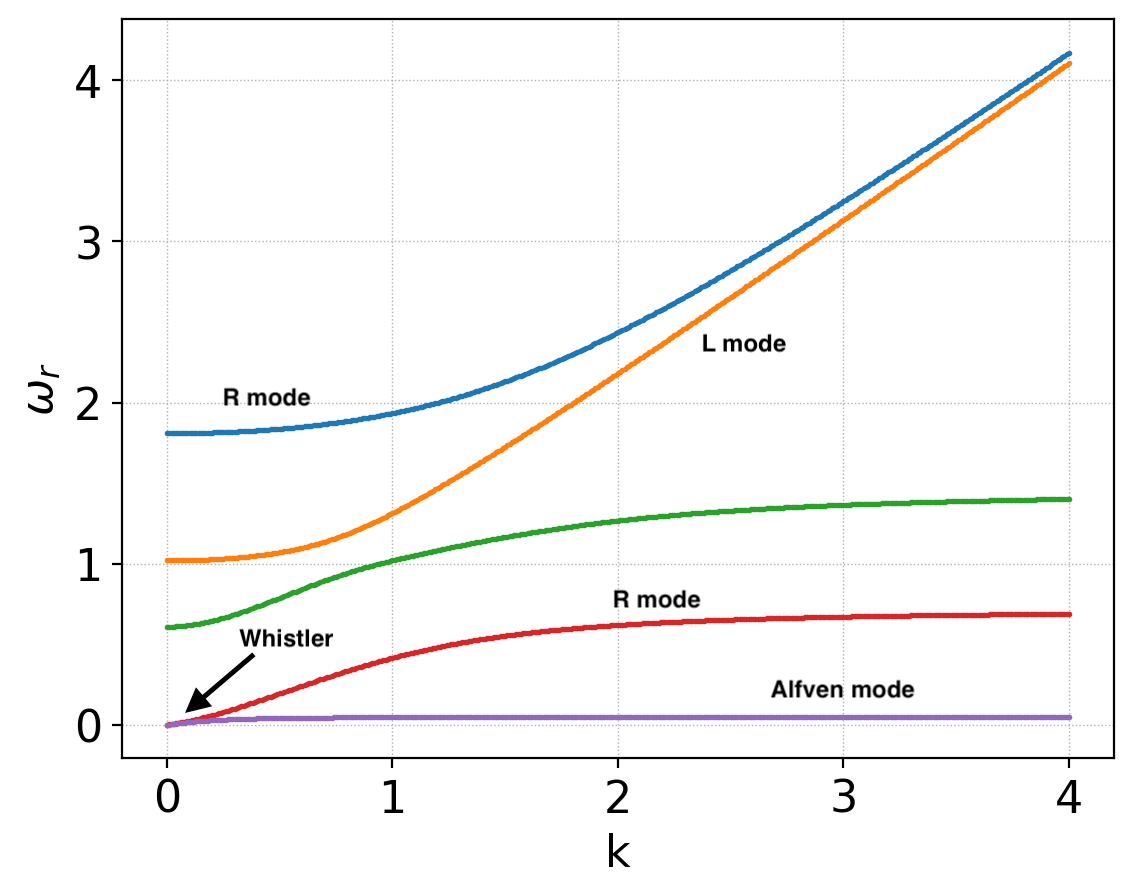
\includegraphics[width=\linewidth]{iso-cold-waves.png}
      \end{figure}
    \end{column}
  \end{columns}
  
\end{frame}

\begin{frame}{Essence of the finite-volume method}
  \small%
  Consider a PDE of the form (non necessarily hyperbolic)
  \begin{align*}
    \pfrac{\mvec{Q}}{t} + \pfrac{\mvec{F}}{x} = 0.    
  \end{align*}
  Now make a grid with cells $I_j = [x_{j-1},x_{j+1/2}]$ and
  $\Delta x = x_{j+1/2} - x_{j-1/2}$. The finite-volume method
  \emph{usually} evolves the cell-averages of the solution:
  \begin{align*}
    \pfrac{\mvec{Q}_j}{t} + \frac{\mvec{F}_{j+1/2} -\mvec{F}_{j-1/2} }{\Delta x} = 0
  \end{align*}
  where
  \begin{align*}
    \mvec{Q}_j(t) \equiv \frac{1}{\Delta x}\int_{I_j} \mvec{Q}(x,t) \thinspace dx
  \end{align*}
  are the \emph{cell-averages} and
  \begin{align*}
    \mvec{F}_{j\pm 1/2} \equiv \mvec{F}(\mvec{Q}_{j\pm 1/2})
  \end{align*}
  are \emph{numerical fluxes} at cell interfaces.

\end{frame}

\begin{frame}{Essence of the finite-volume method}
  \small%
  The finite-volume method \emph{usually} evolves the cell-averages of
  the solution:
  \begin{align*}
    \pfrac{\mvec{Q}_j}{t} + \frac{\mvec{F}_{j+1/2} -\mvec{F}_{j-1/2} }{\Delta x} = 0
  \end{align*}
  This equation is an \emph{exact} evolution equation for the
  cell-averages.\mypause%
  However, notice that
  \begin{itemize}
  \item We only know cell-averages $\mvec{Q}_{j}$ in each cell; we
    \emph{do not} know the \emph{cell-edge} values
    $\mvec{Q}_{j\pm 1/2}$ needed to compute the numerical flux
    $\mvec{F}_{j\pm 1/2}$.%
    \mypause%
  \item The finite-volume method consists of determining these
    \emph{edge values} and \emph{constructing a numerical-flux} so the
    cell-averages can be updated.
  \item Time-stepping can be done with a ODE solver (method-of-lines)
    or using a \emph{single-step} method (fully discrete scheme).
  \end{itemize}
  
\end{frame}

\begin{frame}{Essence of the finite-volume method}
\begin{columns}
  
  \begin{column}{0.5\linewidth}
    Instead of computing one edge value we will compute \emph{two}
    values: one the left and one on right of cell. With this, the
    numerical-flux will then be
    \begin{align*}
      \mvec{F}_{j+1/2} = \mvec{F}_{j+1/2}(\mvec{Q}^{-}_{j+1/2},\mvec{Q}^{+}_{j+1/2})
    \end{align*}
    We must impose the consistency condition:
    \begin{align*}
      \mvec{F}_{j+1/2}(\mvec{Q},\mvec{Q})
      = \mvec{F}(\mvec{Q}).
    \end{align*}
  \end{column}
  
  \begin{column}{0.5\linewidth}
    \begin{figure}    
    \setkeys{Gin}{width=1.0\linewidth,keepaspectratio}
    \incfig{FV-1D-grid.pdf}
  \end{figure}    
  \end{column}
\end{columns}  
\end{frame}

\begin{frame}{Cell-averages v/s cell-center values}
  \small%
  \begin{itemize}
  \item Typically, finite-volume schemes evolve the cell-average
    values; finite-difference schemes evolve cell-center (or nodal)
    values.%
    \mypause%
  \item For some low-order (first and some second-order) schemes the
    \emph{forms} of the scheme may look superficially the
    same. However, this is not true in general and one must \emph{very
      carefully} distinguish between cell-average and point-wise
    values. Otherwise incorrect schemes can result that ``look okay''
    but do not achieve full accuracy.%
    \mypause%
  \item What we evolve (cell-average, nodal values or in DG moments or
    interior node values) is called the \emph{solution
      representation}.
  \end{itemize}
  \begin{block}{Remember Your Representation}
    When studying or designing numerical schemes {\bf never} confuse
    one solution representation for another.
  \end{block}  
\end{frame}

\end{document}


\begin{frame}{}
\end{frame}

\begin{columns}
  
  \begin{column}{0.6\linewidth}
  \end{column}
  
  \begin{column}{0.4\linewidth}
    \includegraphics[width=\linewidth]{fig/Kinsey_2011_Pfus_vs_T.pdf}
  \end{column}
\end{columns}

% ----------------------------------------------------------------
